
\documentclass[12pt,onecolumn]{article}
\usepackage[brazilian]{babel}
\usepackage[utf8]{inputenc}
\usepackage{hyperref}
\usepackage[section]{placeins}
\usepackage{graphicx}
\usepackage{caption}
\usepackage{subcaption}
\usepackage{float}
\usepackage{framed,color}
\usepackage{wrapfig}

\begin{document}

% Title page.
\begin{titlepage}

    % Title info.
    \title{
        \bf
        \LARGE Apostila de \\
        \Huge  Infográficos
    }
    
    \author{Renan Teruo Carneiro \\ Wilson Kazuo Mizutani}
    
    % Print title.
    \maketitle
    
    % No numbering on this page.
    \thispagestyle{empty}
    
\end{titlepage}

\begin{center}
  Copyright (C) 2013 USPGameDev
\end{center}
\begin{figure}[ht]
  \centering
  
\includegraphics[width=\textwidth]{CC-BY.png}
\end{figure}

\vspace{300pt}

Escrito por:
\begin{itemize}
  \item \textbf{Renan Teruo Carneiro} \textit{(imano\_ob at uspgamedev.org)}
  \item \textbf{Wilson Kazuo Mizutani} \textit{(kazuo at uspgamedev.org)}
\end{itemize}

% Page break.
\clearpage

% Print table of contents.
\tableofcontents

% Page break.
\clearpage

\section{Introdução}
  Infográficos são representações gráficas e visuais de informação, dados ou
  conhecimento. Seu objetivo é apresentar informações complexas
  eficientemente\footnotemark.
  
  \footnotetext{
    \url{http://en.wikipedia.org/wiki/Infographic}, acesso em 21/04/2013.
  }
  
  Na realidade, Infográficos já existem há muitos anos. Mas foi só recentemente
  que a proliferação de ferramentas simples e livres trouxeram a criação de
  Infográficos para o alcance de um segmento maior da socedade. É no uso de
  algumas dessas ferramentas que essa apostila se concentra. Não é nosso
  objetivo dar nenhum curso sobre coleta e processamento de dados, mas sim sobre
  as possíveis maneiras de se apresentá-los em seu blog ou site de maneira
  simples e elegante.
  
  Mais particularmente, trabalharemos usando o software livre WordPress como
  ferramenta de blog para publicar os infográficos gerados pelas ferramentas que
  apresentaremos.

\clearpage
\section{\textit{Embedding}}
  Antes de mostrar as ferramentas de infográficos, vamos discutir como elas são
  integradas em um site. Usa-se uma técnica chamada \textit{Embedding}, que se
  traduz mais ou menos como "incorporar". E, de fato, o que essa técnica faz é
  incorporar mídias externas em um site qualquer.
  
  \subsection{Por que precisamos disso?}
    Os infográficos que faremos ficam hospedados no site que os gerou, porque
    eles que possuem a tecnologia para gerá-los. Além disso, serão infográficos
    relativamente interativos, portanto eles não são simples imagens para
    fazermos \textit{download}.
    
    Então, através do \textit{Embedding}, nós fazemos mídias complexas geradas
    em outros sites aparecerem naturalmente no nosso próprio site.
  
  \subsection{Como isso funciona?}
    Talvez você já saiba, mas todas páginas Web possuem um código fonte em
    \textit{HyperText Markup Language} (HTML). Tudo que aparece em uma página
    tem um código HTML por trás. Logo, se queremos colocar um infográfico em
    uma página, precisamos de algum tipo código HTML.
    
    É nesse ponto que entram as ferramentas de infografia Web. Elas não só os
    constroem, como os mantêm hospedados em seus sites e fornecem um trecho de
    código HTML para \textit{Embedding}, isso é, para colocarmos no nosso site.
    Basta copiar tal trecho e colá-lo no código do site, e pronto!
    
  \subsection{Onde eu acesso o código HTML do meu site? Como eu faço um site?}
    Normalmente, contrata-se um \textit{WebMaster} para criar uma página Web, e
    ele fornece um meio de inserirmos código HTML nele. Mas, para simplificar
    essa apostila, e manter o foco no que realmente interessa, usaremos a
    ferramenta de blog WordPress, que faz tudo isso para a gente.
    
    Nesse caso, você tem duas opções: criar um blog hospedado em
    \url{www.wordpress.com}, ou pedir para os monitores do curso criarem um
    para você\footnotemark. Uma vez que você tenha seu próprio WordPress, você
    poderá inserir código HTML nos seus \textit{posts} do blog, apresentando os
    infográficos que quiser.
    
    \footnotetext{
      Normalmente no endereço \url{www.uspgamedev.org/cursos/wordpress/}.
    }

\clearpage
\section{Datawrapper}
  \url{http://datawrapper.de/}

\clearpage
\section{Infogram}
  \textbf{Endereço: \url{http://infogr.am/}}
  
  Infogram é um site de serviço Web voltado para a criação e manutenção de
  infográficos dos mais diversos tipos, relativamente interativos e com
  aparência profissional. Seu uso não exige nenhum tipo de conhecimento de
  design, apenas uma noção elementar de manipulação de planilhas. O site fornece
  um cadastro gratuito, com possibilidade de adquirir uma conta "Pro" para ter
  acesso a funcionalidades avançadas.
  
  Uma vez feita uma conta, é possível começar imediatamente a fazer
  infográficos. Na verdade, o site permite você criar um \textit{layout}
  bastante completo contendo um ou mais infográficos, textos, citações, imagens,
  mapas e vídeos. Também existem vários temas para esses \textit{layouts}.
  
  Na primeira vez que você entrar, o Infogr.am mostrará um esquema rápido
  explicando o que é cada ferramenta. Não são muitas, é bem simples de entender.
  A interface é dividida em quatro partes:
  
  \begin{itemize}
    \item
      \textbf{Menu lateral esquerdo:}
      Controle da conta, acesso à biblioteca pessoal de
      infográficos.
    \item
      \textbf{Menu lateral direito:}
      Adiciona elementos no \textit{layout} que você quer
      publicar, em particuar cria os infográficos.
    \item
      \textbf{Menu superior:}
      Configurações do \textit{layout}, prévia visual do resultado,
      \textit{download} (funcionalidade para contas Pro) e compartilhar. É nessa
      última opção ("\textit{share}") que você poderá obter o código HTML para
      incorporar sua produção no seu site.
    \item
      \textbf{Editor visual do \textit{layout}:}
      Aqui você pode posicionar os elementos do seu \textit{layout}, escrever
      textos neles e colocar uma nota de \textit{Copyright}. Quando você clicar
      duas vezes em um infográfico, um menu de edição aparecerá para você mudar
      as configurações e os dados usados por ele.
  \end{itemize}
  
  Os dados usados pelos infográficos devem ser fornecidos em uma planilha, o que
  é bastante conveniente. No entanto, esses dados precisam já estar processados
  e distribuídos da maneira que o Infogr.am espera. Por exemplo, um gráfico de
  linhas espera por uma tabela com: uma coluna com identificadores para cada
  linha do gráfico, e várias colunas com os valores associados acada
  identificador ao longo do tempo.
  
  \begin{figure}[H]
    \centering
    \begin{subfigure}{\textwidth}
      \centering
      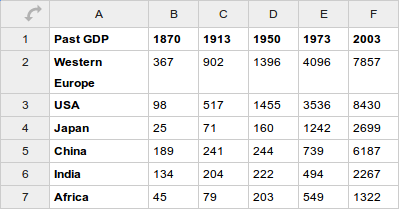
\includegraphics[width=.9\linewidth]{infogram-sample-spreadsheet.png}
      \label{fig:infogram-sample-spreadsheet}
    \end{subfigure}
    \begin{subfigure}{\textwidth}
      \centering
      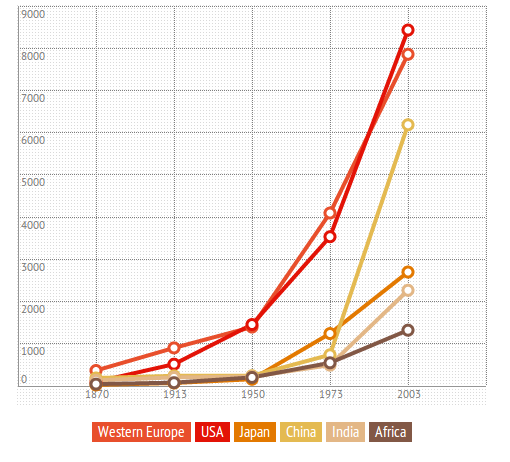
\includegraphics[width=.9\linewidth]{infogram-sample-chart.png}
      \label{fig:infogram-sample-chart}
    \end{subfigure}
    \caption{
      \footnotesize
      \it
      Exemplo de planilha que o Infogr.am usa, e o infográfico resultante.
    }
  \end{figure}

\clearpage
\section{Google Trends}
  \url{http://www.google.com/trends/}

\clearpage
\section{Wordle}
  \url{http://www.wordle.net/}

\end{document}
